% какие-то дополнения:
% $\gamma(t)$ — гладкая, регулярная.
% $\gamma'(t)$ — вектор скорости кривой.
% $||\gamma'(t)|| > 0$ (из регулярности)
% $$S = \int_{0}^{t} ||\gamma'(u)|| \,du$$
% $$||\frac{d\gamma}{ds}|| = 1$$

% $$\int_{0}^{a} ||\gamma'(u)|| \,du$$ — длина кривой между точками $\gamma(0)$ и $\gamma(a)$.

\begin{statement}
    Пусть дана регулярная кривая $\gamma(t)$, тогда кривая, полученная из данной с помощью параллельного переноса, поворота или гомотетии, ей регулярно гомотопна.
\end{statement} 
\begin{proof}\tab
    \begin{itemize}
        \item Параллельный перенос: 
        $$\gamma(t) \to \gamma(t) + w \Longrightarrow \gamma(t,s) = \gamma(t) + sw$$

        \item Поворот: 
        $$\gamma(t) \to \begin{pmatrix}
            \cos{\phi_0} & -\sin{\phi_0} \\
            \sin{\phi_0} & \cos{\phi_0}
        \end{pmatrix} \gamma(t)
        \Longrightarrow
        \gamma(t,s) = \begin{pmatrix}
            \cos{\phi_0 s} & -\sin{\phi_0 s} \\
            \sin{\phi_0 s} & \cos{\phi_0 s}
        \end{pmatrix} \gamma(t)$$

        \item Гомотетия: $$\gamma(t) \to \mu \gamma(t) \Longrightarrow \gamma(t,s) = (1 - s + \mu s) \gamma(t), \ s \in [0,1]$$
    \end{itemize}
\end{proof} 

Подготовительные утверждения к теореме Уитни доказаны: теперь мы можем регулярной гомотопией заменить кривые $\gamma_0(t)$ и $\gamma_1(t)$ на кривые, которые расположены так, как нам удобно (их можно поворачивать, сдвигать, растягивать), причём вектор скорости у полученных кривых будет единичной длины.

\begin{proof}[Доказательство теоремы Уитни]
    $\underline{\Longrightarrow}$ 
    Если кривые $\gamma_0(t)$ и $\gamma_1(t)$ регулярно гомотопны, то число вращения $R(\gamma_s)$ непрерывно зависит от параметра гомотопии $s$ (поскольку $\phi_s(t)$ непрерывно по $s$).

    Так как $R(\gamma_s) \in \Z$, то оно не меняется в процессе гомотопии, поэтому $R(\gamma_1) = R(\gamma_2)$.

    $\underline{\Longleftarrow}$ 
    Пусть $\gamma_0(t)$ и $\gamma_1(t)$ — замкнутые регулярные кривые, $\gamma_i(t): [0,T] \to \R^2$ такие, что $R(\gamma_0) = R(\gamma_1)$.

    Считаем, что параметр на кривых натуральный:
    \[\left|\frac{d\gamma_0}{dt}\right| \equiv \left|\frac{d\gamma_1}{dt}\right| \equiv 1\]
    и кривые заданы на одном и том же отрезке $t \in [0,T]$.

    Расположим кривые так, как нам удобно: пусть в начальный момент времени кривые $\gamma_0(t)$ и $\gamma_1(t)$ проходят через начало координат: $\gamma_0(0) = \gamma_1(0) = (0,0)$ и имеют один и тот же касательный вектор $(1,0)$:
    \[\frac{d\gamma_0}{dt}(0) = \frac{d\gamma_1}{dt}(0) = (1,0).\]

    \begin{figure}[ht]
        \centering
        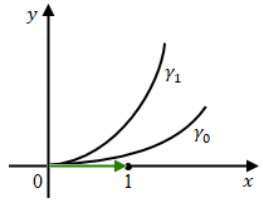
\includegraphics[scale=0.7]{images/c13.1.png}
        \caption{Кривые $\gamma_0(t)$ и $\gamma_1(t)$.}
        \label{fig:c13.1}
    \end{figure}

    Докажем теперь, что кривые $\gamma_0$ и $\gamma_1$ регулярно гомотопны, при условии, что их числа вращения равны $R(\gamma_0) = R(\gamma_1)$.

    Поскольку вектор скорости имеет единичную длину, то можно считать, что
    \[\frac{d\gamma_0}{dt} = (\cos{\phi_0(t)}, \sin{\phi_0(t)}),\]
    \[\frac{d\gamma_1}{dt} = (\cos{\phi_1(t)}, \sin{\phi_1(t)}),\]
    где $\phi_0(t), \ \phi_1(t)$ — непрерывные функции.

    Так как числа вращения кривых равны, то $\phi_0(T) = \phi_1(T) = 2\pi k$, где $k$ — число вращения. Также $\phi_0(0) = \phi_1(0) = 0$ (мы так расположили кривые).

    Тогда построим гомотопию между функциями $\phi_0(t)$ и $\phi_1(t)$:
    \[\phi_s(t) = (1-s) \phi_0(t) + s \phi_1(t).\]
    Будем считать $\phi_s(t)$ тоже функцией угла, задающей единичный вектор $v_s(t)$:
    \[v_s(t) = (\cos{\phi_s(t)}, \sin{\phi_s(t)}).\]
    Будем также считать $v_s(t)$ вектором скорости некоторой кривой $\tilde{\gamma_s}(t)$ — её нужно немного видоизменить, чтобы получить то семейство кривых, которое мы строим для гомотопии между $\gamma_0$ и $\gamma_1$.

    Так как $\tilde{\gamma_s}(0) = (0,0)$, то 
    \[\tilde{\gamma_s}(t) = \int_{0}^{t} v_s(\tau) \, d\tau\]
    — построили некоторое семейство кривых. Ясно, что при $s = 0$ мы получим кривую $\gamma_0(t)$, при $s = 1$ — кривую $\gamma_1(t)$.

    Кривая $\tilde{\gamma_s}(t)$, очевидно, регулярна (длина вектора скорости равна 1), но она может быть незамкнутой — равенство функций $\phi_s(t)$ и $v_s(t)$ при $t=0$ и $t=T$ означает, что в начальной и конечной точке кривой одинаковый вектор скорости (см.рис.\ref{fig:c13.2}).

    \begin{figure}[ht]
        \centering
        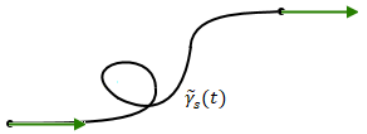
\includegraphics[scale=0.7]{images/c13.2.png}
        \caption{Кривая $\tilde{\gamma_s}(t)$ может быть незамкнутой.}
        \label{fig:c13.2}
    \end{figure}

    Немного изменим кривую $\tilde{\gamma_s}(t)$, чтобы она стала замкнутой. Рассмотрим радиус-вектор новой кривой: пусть его конечная точка пробегает кривую $\tilde{\gamma_s}(t)$, а начальная точка пробегает отрезок, соединяющий начало и конец $\tilde{\gamma_s}(t)$ (см.рис.\ref{fig:c13.3}).

    \begin{figure}[ht]
        \centering
        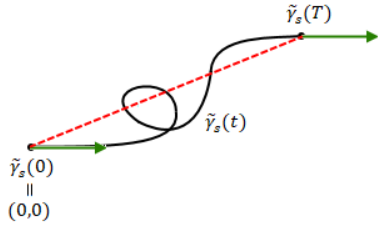
\includegraphics[scale=0.7]{images/c13.3.png}
        \caption{Построение $\gamma_s(t)$.}
        \label{fig:c13.3}
    \end{figure}

    Получим 
    \[\gamma_s(t) = \tilde{\gamma_s}(t) - \frac{t}{T} \tilde{\gamma_s}(T).\]
    Примем эту формулу за определение семейства кривых, связывающих кривые $\gamma_0$ и $\gamma_1$ (иными словами, за отображение $\gamma(s,t)$ из определения гомотопии).

    Действительно, так как $\gamma_0$ и $\gamma_1$ замкнутые и $\gamma_0(T) = \gamma_1(T) = (0,0)$, то при $s=0$ получаем $\gamma_0(t)$, при $s=1$ — $\gamma_1(t)$.

    Проверим, что при любом значении параметра $s$ кривая $\gamma_s(t)$ замкнута и регулярна.
    
    Замкнутость: при $t=0$ получаем $\tilde{\gamma_s}(0) = 0$, при $t=T$ получаем $\tilde{\gamma_s}(T) - \tilde{\gamma_s}(T) = 0$.
    
    Регулярность: проверим, что
    \[\frac{d\gamma_s(t)}{dt} \neq 0.\]
    В самом деле (учтём, что кривая $\tilde{\gamma_s}(t)$ строилась так, что её вектор скорости $\frac{d\tilde{\gamma_s}(t)}{dt} = 1$):

    \begin{multline*}
        \left|\frac{d\gamma_s(t)}{dt}\right| = \left|\frac{d\tilde{\gamma_s}(t)}{dt} - \frac{1}{T}\tilde{\gamma_s}(T)\right| \geqslant \left|\frac{d\tilde{\gamma_s}(t)}{dt}\right| - \frac{1}{T} \left|\tilde{\gamma_s}(T)\right| =\\ 
        = 1 - \frac{1}{T} \left|\tilde{\gamma_s}(T)\right| = \frac{T - \left|\tilde{\gamma_s}(T)\right|}{T} \geqslant 0.
    \end{multline*} 

    Для того, чтобы кривая была регулярной, неравенство должно быть строгим. Вначале поймём, почему нестрогие неравенства выполняются: $T$ — это длина кривой $\tilde{\gamma_s}(t)$ (на ней выбран натуральный параметр), а длина вектора $\tilde{\gamma_s}(T)$ — это длина отрезка, соединяющего начальную и конечную точки кривой $\tilde{\gamma_s}(t)$ (см.рис.\ref{fig:c13.3}).
    Поэтому геометрически последнее неравенство выражает тот факт, что длина кривой, соединяющей эти точки, не меньше, чем длина отрезка, соединяющего эти точки.

    Более формально неравенство 
    \[\frac{T - \left|\tilde{\gamma_s}(T)\right|}{T} \geqslant 0\]
    можно доказать воспользовавшись тем, что интеграл от модуля функции не меньше модуля интеграла функции:
    \begin{multline*}
        T = \int_{0}^{T}1 \, dt = \int_{0}^{T} \left|\frac{d\tilde{\gamma_s}(t)}{dt}\right| \, dt \geqslant \left|\int_{0}^{T}\frac{d\tilde{\gamma_s}(t)}{dt} \, dt\right| = \left|\tilde{\gamma_s}(T) - \tilde{\gamma_s}(0)\right| = \left|\tilde{\gamma_s}(T)\right|.
    \end{multline*} 

    Равенство будет достигаться только в случае, когда кривая совпадает с отрезком. Иначе говоря, неравенства «$\geqslant$» обращаются в равенства только в том случае, когда $\phi_s(t) \equiv 0$ (действительно, если вектора скорости в любой точке кривой коллинеарны, то $v_s(t) \equiv 0$, откуда следует, что $\phi_s(t) \equiv 0$).

    Иными словами, во всех случаях, кроме случая, когда для некоторого $s$ выполнено $\phi_s(t) \equiv 0$, теорема доказана, потому что мы явно предъявили гомотопию.

    В случае когда для некоторого $s$ выполнено $\phi_s(t) \equiv 0$, функции $\phi_0(t)$ и $\phi_1(t)$ имеют специальный вид: они связаны линейной зависимостью 
    \[\phi_s(t) = (1-s)\phi_0(t) + s\phi_1(t).\]

    В этом случае мы с помощью регулярной гомотопии можем изменить одну из функций, и линейная зависимость между ними пропадёт (см.рис.\ref{fig:c13.4}).

    \begin{figure}[ht]
        \centering
        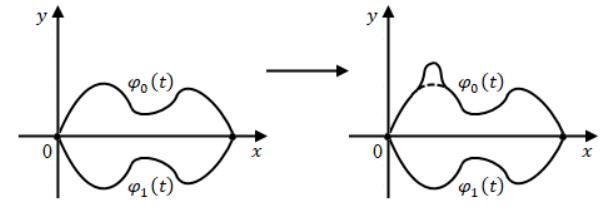
\includegraphics[scale=0.7]{images/c13.4.png}
        \caption{Функции $\phi_0(t)$ и $\phi_1(t)$ линейно зависимы ($s = 0.5$).}
        \label{fig:c13.4}
    \end{figure}


    Далее способом, описанным выше, построим регулярную гомотопию между новой (возмущённой) кривой $\phi_0(t)$ и кривой $\phi_1(t)$. Таким образом (ура), теорема Уитни доказана.
\end{proof} 

\subsection{Регулярные замкнутые кривые на двумерной сфере}
Наша задача состоит в том, чтобы выяснить, когда две регулярные замкнутые кривые на сфере являются регулярно гомотопными.

Проблема состоит в том, что теория гладких многообразий обсуждается в курсе дифференциальной геометрии, поэтому дать определение регулярной кривой на сфере довольно проблематично. Мы обойдёмся простыми случаями.

В первых главах разбиралась стереографическая проекция (сюда бы ссылку). Так как сфера без северного полюса гомеоморфна плоскости, то гладкие кривые на сфере можно рассматривать как гладкие в координатах, которые получаются при соответствии между точками сферы и точками плоскости (будем считать, что кривые не проходят через северный полюс).

Также можем считать, что замкнутая регулярная кривая расположена на «небольшом» участке сферы и (по теореме Уитни для плоскости) регулярно гомотопна кривой вида, изображённого на рисунке \ref{fig:c13.5}.

\begin{figure}[ht]
    \centering
    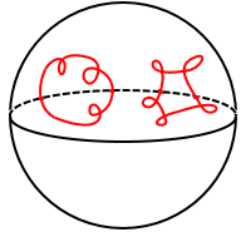
\includegraphics[scale=0.7]{images/c13.5.png}
    \caption{Замкнутые регулярные кривые на сфере.}
    \label{fig:c13.5}
\end{figure}

То есть, число классов регулярной гомотопии может только уменьшиться — может оказаться, что кривые, которые на плоскости не были регулярно гомотопными, на сфере окажутся регулярно гомотопными.

Действительно, на сфере нельзя определить число вращения кривой (так как на плоскости мы можем измерить угол между вектором скорости кривой и каким-то фиксированным направлением, например, осью $x$, а на сфере не существует способа задать фиксированное направление во всех точках сразу).

Но мы всегда можем рассуждать следующим образом: можно считать, что кривая находится на небольшом участке сферы, которые гомеоморфен плоскости. Значит, можно вычислить «число вращения», затем регулярной гомотопией как-то изменить кривую, затем снова перетащить её на этот участок сферы и опять вычислить «число вращения» — в процессе оно может меняться.

Рассмотрим процесс удаления двух соседних петелек: вытягивая кривую по сфере, придём к участку кривой, содержащему петельки с другой стороны (см.рис.\ref{fig:c13.6}).

\begin{figure}[ht]
    \centering
    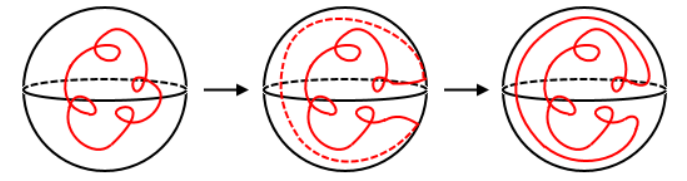
\includegraphics[scale=0.7]{images/c13.6.png}
    \caption{Удаление соседних петелек у кривой на сфере.}
    \label{fig:c13.6}
\end{figure}

Если «число вращения» кривой до совершения этой операции было равно $k+1$, то «число вращения» после совершения операции будет равно $k-1$ (по определению — посчитаем количество оборотов вектора скорости при движении точки по кривой).

Итак, после такой гомотопии «число вращения» изменится на 2. Отсюда следует, что кривые, у которых «число вращения» отличается на 2, регулярно гомотопны. Поэтому на сфере останется всего два класса регулярной гомотопности.

\begin{statement}
    На сфере существует ровно два класса гладких регулярных замкнутых кривых с точностью до регулярной гомотопии (на плоскости, кстати, их счётное число).
\end{statement} 

\begin{theorem}
    Любая замкнутая кривая на сфере регулярно гомотопна либо «окружности», либо «восьмёрке», направление обхода при этом неважно.
\end{theorem} 